\documentclass{beamer}

%
% Common preamble for all three parts.
%

\usepackage[spanish]{babel}
\usepackage{amsmath}
\usepackage{color}
\ProvidesPackage{minted}
\usepackage{minted}
%\setminted{encoding=utf8}
\usepackage{hyperref}
\usepackage{multicol}
\usepackage{tabularx}
\usepackage{tikz}

\usepackage[utf8x]{inputenc}
%\usepackage{ucs}
%\usepackage[T1]{fontenc}
%\newcommand{\minted@encoding}{\minted@get@opt{encoding}{UTF8}}

\usepackage{verbatim}
\usepackage{fancyvrb}
\usepackage{listings}

\lstset{
  basicstyle=\tiny, language=c,
  keywordstyle=\color{purple}\bfseries,
  morekeywords={printf}, frame=shadowbox,
  breaklines=true, rulesepcolor=\color{purple},
  numbers=left, stringstyle=\ttfamily,
  fancyvrb=false}

\usepackage[american,cuteinductors,siunitx,rotatelabels]{circuitikz}
\usepackage{siunitx}

% only inline todonotes work
\usepackage{xkeyval}
\usepackage[textsize=small]{todonotes}
\presetkeys{todonotes}{inline}{}

\usetikzlibrary{shapes,arrows,positioning,shadows}

% no nav buttons
\usenavigationsymbolstemplate{}

\newcommand{\bftt}[1]{\textbf{\texttt{#1}}}
%FIXED presentaba conflictos con los paquetes agregados para la Parte 4  \newcommand{\comment}[1]{{\color[HTML]{008080}\textit{\textbf{\texttt{#1}}}}}
\newcommand{\cmd}[1]{{\color[HTML]{008000}\bftt{#1}}}
\newcommand{\bs}{\char`\\}
\newcommand{\cmdbs}[1]{\cmd{\bs#1}}
\newcommand{\lcb}{\char '173}
\newcommand{\rcb}{\char '175}
\newcommand{\cmdbegin}[1]{\cmdbs{begin\lcb}\bftt{#1}\cmd{\rcb}}
\newcommand{\cmdend}[1]{\cmdbs{end\lcb}\bftt{#1}\cmd{\rcb}}

\newcommand{\wllogo}{\textbf{Overleaf}}

% this is where the example source files are loaded from
% do not include a trailing slash
\newcommand{\fileuri}{https://raw.github.com/guanucoluis/latex-course/master/es}

\newcommand{\wlserver}{https://www.overleaf.com}
\newcommand{\wlnewdoc}[1]{\wlserver/docs?snip\_uri=\fileuri/#1\&splash=none}

\def\tikzname{Ti\emph{k}Z}

% from http://tex.stackexchange.com/questions/5226/keyboard-font-for-latex
\newcommand*\keystroke[1]{%
  \tikz[baseline=(key.base)]
    \node[%
      draw,
      fill=white,
      drop shadow={shadow xshift=0.25ex,shadow yshift=-0.25ex,fill=black,opacity=0.75},
      rectangle,
      rounded corners=2pt,
      inner sep=1pt,
      line width=0.5pt,
      font=\scriptsize\sffamily
    ](key) {#1\strut}
  ;
}
\newcommand{\keystrokebftt}[1]{\keystroke{\bftt{#1}}}

% stolen from minted.dtx
\newenvironment{exampletwoup}
  {\VerbatimEnvironment
   \begin{VerbatimOut}{example.out}}
  {\end{VerbatimOut}
   \setlength{\parindent}{0pt}
   \fbox{\begin{tabular}{l|l}
   \begin{minipage}{0.55\linewidth}
     \inputminted[fontsize=\small,resetmargins]{latex}{example.out}
   \end{minipage} &
   \begin{minipage}{0.35\linewidth}
     \input{example.out}
   \end{minipage}
   \end{tabular}}}

\newenvironment{exampletwouptiny}
  {\VerbatimEnvironment
   \begin{VerbatimOut}{example.out}}
  {\end{VerbatimOut}
   \setlength{\parindent}{0pt}
   \fbox{\begin{tabular}{l|l}
   \begin{minipage}{0.55\linewidth}
     \inputminted[fontsize=\scriptsize,resetmargins]{latex}{example.out}
   \end{minipage} &
   \begin{minipage}{0.35\linewidth}
     \setlength{\parskip}{6pt plus 1pt minus 1pt}%
     \raggedright\scriptsize\input{example.out}
   \end{minipage}
   \end{tabular}}}

\newenvironment{exampletwouptinynoframe}
  {\VerbatimEnvironment
   \begin{VerbatimOut}{example.out}}
  {\end{VerbatimOut}
   \setlength{\parindent}{0pt}
   \begin{tabular}{l|l}
   \begin{minipage}{0.55\linewidth}
     \inputminted[fontsize=\scriptsize,resetmargins]{latex}{example.out}
   \end{minipage} &
   \begin{minipage}{0.35\linewidth}
     \setlength{\parskip}{6pt plus 1pt minus 1pt}%
     \raggedright\scriptsize\input{example.out}
   \end{minipage}
   \end{tabular}}

\title{Una Introducción Interactiva a \LaTeX}
\author{Siria Sadeddin}
 %este preábulo es agregado por guanucoluis

\subtitle{Parte 4: Adaptando el documento a nuestras necesidades}

\begin{document}

%%%%%%%%%%%%%%%%%%%%%%%%%%%%%%%%%%%%%%%%%%%%%%%%%%%%%%%%%%%%%%%%%%%%%%%%%%%%%%%
%%%%%%%%%%%%%%%%%%%%%%%%%%%%%%%%%%%%%%%%%%%%%%%%%%%%%%%%%%%%%%%%%%%%%%%%%%%%%%%
%%%%%%%%%%%%%%%%%%%%%%%%%%%%%%%%%%%%%%%%%%%%%%%%%%%%%%%%%%%%%%%%%%%%%%%%%%%%%%%
\begin{frame}
  \titlepage
\end{frame}

%%%%%%%%%%%%%%%%%%%%%%%%%%%%%%%%%%%%%%%%%%%%%%%%%%%%%%%%%%%%%%%%%%%%%%%%%%%%%%%
%%%%%%%%%%%%%%%%%%%%%%%%%%%%%%%%%%%%%%%%%%%%%%%%%%%%%%%%%%%%%%%%%%%%%%%%%%%%%%%
%%%%%%%%%%%%%%%%%%%%%%%%%%%%%%%%%%%%%%%%%%%%%%%%%%%%%%%%%%%%%%%%%%%%%%%%%%%%%%%
\section{Estilo De Las Páginas}

%%%%%%%%%%%%%%%%%%%%%%%%%%%%%%%%%%%%%%%%%%%%%%%%%%%%%%%%%%%%%%%%%%%%%%%%%%%%%%%
%%%%%%%%%%%%%%%%%%%%%%%%%%%%%%%%%%%%%%%%%%%%%%%%%%%%%%%%%%%%%%%%%%%%%%%%%%%%%%%
%%%%%%%%%%%%%%%%%%%%%%%%%%%%%%%%%%%%%%%%%%%%%%%%%%%%%%%%%%%%%%%%%%%%%%%%%%%%%%%
\begin{frame}[fragile]{\insertsection: Nativos}
  \begin{itemize}
  \item \LaTeX{} soporta diferentes combinaciones de cabeceras y
    pies de páginas. \cmdbs{pagestyle} define cuál emplearse.
    \begin{itemize}
    \item \bftt{empty}
    \item \bftt{plain}
    \item \bftt{headings}      
    \item \bftt{myheadings}      
    \end{itemize}
  \item Es posible cambiar el estilo de la página actual con la orden
    pies de páginas \cmdbs{thispagestyle}.
  \end{itemize}
\end{frame}

%%%%%%%%%%%%%%%%%%%%%%%%%%%%%%%%%%%%%%%%%%%%%%%%%%%%%%%%%%%%%%%%%%%%%%%%%%%%%%%
%%%%%%%%%%%%%%%%%%%%%%%%%%%%%%%%%%%%%%%%%%%%%%%%%%%%%%%%%%%%%%%%%%%%%%%%%%%%%%%
%%%%%%%%%%%%%%%%%%%%%%%%%%%%%%%%%%%%%%%%%%%%%%%%%%%%%%%%%%%%%%%%%%%%%%%%%%%%%%% 
\begin{frame}[fragile]{\insertsection: Personalizados}
  El estilo \bftt{myheadings} permite modificar el contenido de
  la cabecera.\\[2ex]
  \begin{minipage}{0.5\linewidth}
    \inputminted[fontsize=\scriptsize,frame=single,resetmargins]{latex}%
    {es/pagestyle-example-myheadings.tex}
  \end{minipage}
  \begin{minipage}{0.4\linewidth}
    % trim: l b r t
    
\includegraphics[width=\textwidth,clip,trim=1in 1.1in 1in 1.1in,page=6]{pagestyle-example-myheadings.pdf}
  \end{minipage}
\end{frame}

%%%%%%%%%%%%%%%%%%%%%%%%%%%%%%%%%%%%%%%%%%%%%%%%%%%%%%%%%%%%%%%%%%%%%%%%%%%%%%% 
%%%%%%%%%%%%%%%%%%%%%%%%%%%%%%%%%%%%%%%%%%%%%%%%%%%%%%%%%%%%%%%%%%%%%%%%%%%%%%%
%%%%%%%%%%%%%%%%%%%%%%%%%%%%%%%%%%%%%%%%%%%%%%%%%%%%%%%%%%%%%%%%%%%%%%%%%%%%%%%

\begin{frame}[fragile]{\insertsection: Personalizados}
  El paquete \bftt{fancyhdr} provee comandos para definir el
  contenido del lado izquierdo, centro y derecho, tanto del
  encabezado como el pie de página.\\[2ex]
  \begin{minipage}{0.5\linewidth}
    \inputminted[fontsize=\tiny,frame=single,resetmargins]{latex}%
    {es/pagestyle-example-fancyhdr.tex}
  \end{minipage}
  \begin{minipage}{0.4\linewidth}
    % trim: l b r t
    
\includegraphics[width=\textwidth,clip,trim=1in 1.1in 1in 1.1in,page=6]{pagestyle-example-fancyhdr.pdf}
  \end{minipage}
\end{frame}

%%%%%%%%%%%%%%%%%%%%%%%%%%%%%%%%%%%%%%%%%%%%%%%%%%%%%%%%%%%%%%%%%%%%%%%%%%%%%%%
%%%%%%%%%%%%%%%%%%%%%%%%%%%%%%%%%%%%%%%%%%%%%%%%%%%%%%%%%%%%%%%%%%%%%%%%%%%%%%%
%%%%%%%%%%%%%%%%%%%%%%%%%%%%%%%%%%%%%%%%%%%%%%%%%%%%%%%%%%%%%%%%%%%%%%%%%%%%%%%

\section{Código Fuente en \LaTeX}

%%%%%%%%%%%%%%%%%%%%%%%%%%%%%%%%%%%%%%%%%%%%%%%%%%%%%%%%%%%%%%%%%%%%%%%%%%%%%%% 
%%%%%%%%%%%%%%%%%%%%%%%%%%%%%%%%%%%%%%%%%%%%%%%%%%%%%%%%%%%%%%%%%%%%%%%%%%%%%%% 
%%%%%%%%%%%%%%%%%%%%%%%%%%%%%%%%%%%%%%%%%%%%%%%%%%%%%%%%%%%%%%%%%%%%%%%%%%%%%%%


\begin{frame}[fragile]{\insertsection: Entorno \bftt{verbatim}}
  \begin{itemize}
  \item El texto encerrado entre \cmdbegin{verbatim} y
    \cmdend{verbatim} se escribirá directamente, con todos los saltos
    de línea y espacios, sin ejecutar ninguna orden \LaTeX.\\[1ex]
    \begin{exampletwouptiny}
\begin{verbatim}
#include<stdio.h>

int main()
{
  printf("Hello World");
  return 0;
}
\end{verbatim}
    \end{exampletwouptiny}
    \vskip 2ex
  \item Dentro de un párrafo, un comportamiento similar se puede 
    obtener con \cmdbs{verb}+text+.
  \end{itemize}
\end{frame}

%%%%%%%%%%%%%%%%%%%%%%%%%%%%%%%%%%%%%%%%%%%%%%%%%%%%%%%%%%%%%%%%%%%%%%%%%%%%%%% 
%%%%%%%%%%%%%%%%%%%%%%%%%%%%%%%%%%%%%%%%%%%%%%%%%%%%%%%%%%%%%%%%%%%%%%%%%%%%%%% 
%%%%%%%%%%%%%%%%%%%%%%%%%%%%%%%%%%%%%%%%%%%%%%%%%%%%%%%%%%%%%%%%%%%%%%%%%%%%%%%


\begin{frame}[fragile]{\insertsection: Paquetes \bftt{verbatim} y \bftt{fancyvrb}}
  \begin{itemize}
  \item El paquete \bftt{verbatim} nos permite incluir un fichero de
    texto como si estuviera dentro de un entorno \bftt{verbatim}.\\[2ex]
    \begin{exampletwouptiny}
\verbatiminput{es/main.c}
    \end{exampletwouptiny}
  \end{itemize}
\end{frame}

%%%%%%%%%%%%%%%%%%%%%%%%%%%%%%%%%%%%%%%%%%%%%%%%%%%%%%%%%%%%%%%%%%%%%%%%%%%%%%% 
%%%%%%%%%%%%%%%%%%%%%%%%%%%%%%%%%%%%%%%%%%%%%%%%%%%%%%%%%%%%%%%%%%%%%%%%%%%%%%% 
%%%%%%%%%%%%%%%%%%%%%%%%%%%%%%%%%%%%%%%%%%%%%%%%%%%%%%%%%%%%%%%%%%%%%%%%%%%%%%%


\begin{frame}[fragile]{\insertsection: Paquetes \bftt{verbatim} y \bftt{fancyvrb}}
  \begin{itemize}
  \item {\small El paquete \bftt{fancyvrb} nos permite incluir un fichero de
      texto como si estuviera dentro de un entorno \bftt{verbatim}.}\\[2ex]
  \item {\small Con el paquete \bftt{fancyvrb} se puede realizar
      tareas comunes a código-fuente, tales como: cambiar la fuente
      del texto y tamaño, numerar las líneas, etc.}\\[2ex]
    \begin{exampletwouptiny}
\VerbatimInput[frame=lines,
fontshape=sl,
fontsize=\scriptsize,
numbers=left,
formatcom=\color{blue}]
{es/main.c}
    \end{exampletwouptiny}

  \end{itemize}
\end{frame}

%%%%%%%%%%%%%%%%%%%%%%%%%%%%%%%%%%%%%%%%%%%%%%%%%%%%%%%%%%%%%%%%%%%%%%%%%%%%%%% 
%%%%%%%%%%%%%%%%%%%%%%%%%%%%%%%%%%%%%%%%%%%%%%%%%%%%%%%%%%%%%%%%%%%%%%%%%%%%%%% 
%%%%%%%%%%%%%%%%%%%%%%%%%%%%%%%%%%%%%%%%%%%%%%%%%%%%%%%%%%%%%%%%%%%%%%%%%%%%%%%


\begin{frame}[fragile]{\insertsection: Paquete \bftt{listings}}
  \begin{itemize}
  \item {\small El paquete \bftt{listings} se utiliza para imprimir
      código-fuente en \LaTeX{}. El entorno es similar al paquete 
      \bftt{verbatim}}.
    \begin{exampletwouptiny}
\begin{lstlisting}
  #include<stdio.h>
  
  int main()
  {
    printf("Hello World");
    return 0;
  }
\end{lstlisting}
    \end{exampletwouptiny}
    \vskip 2ex
  \item {\small Para personalizar el entorno \bftt{listings} se
      utiliza el comando \cmdbs{lstset}. El código siguiente debe ser
      agregado en el preámbulo del archivo \LaTeX{}.}
    \begin{minted}[fontsize=\scriptsize,frame=single]{latex}
\usepackage{listings}
\lstset{
  basicstyle=\tiny, language=c, fancyvrb=false, numbers=left,
  keywordstyle=\color{blue}\bfseries, frame=shadowbox,
  morekeywords={printf}, breaklines=true, 
  rulesepcolor=\color{blue}, stringstyle=\ttfamily}
    \end{minted}
  \end{itemize}
\end{frame}

%%%%%%%%%%%%%%%%%%%%%%%%%%%%%%%%%%%%%%%%%%%%%%%%%%%%%%%%%%%%%%%%%%%%%%%%%%%%%%% 
%%%%%%%%%%%%%%%%%%%%%%%%%%%%%%%%%%%%%%%%%%%%%%%%%%%%%%%%%%%%%%%%%%%%%%%%%%%%%%% 
%%%%%%%%%%%%%%%%%%%%%%%%%%%%%%%%%%%%%%%%%%%%%%%%%%%%%%%%%%%%%%%%%%%%%%%%%%%%%%%


\begin{frame}[fragile]{\insertsection: Paquete \bftt{minted}}
  \begin{itemize}
  \item {\small El paquete \bftt{minted} permite insertar código
      fuente y resaltar las la sintaxis del lenguaje utilizado. Este
      paquete utiliza una librería del lenguaje Python
      (\bftt{python-pygments}).}
    \vskip 2ex
    \begin{exampletwouptiny}
\begin{minted}[fontsize=\tiny,
  frame=single,
  linenos=true]{c}
  #include<stdio.h>
  
  int main()
  {
    printf("Hello World");
    return 0;
  }
\end{minted}
    \end{exampletwouptiny}
    \vskip 2ex
  \item {\small Los últimos dos paquetes, \bftt{listings} y
      \bftt{minted}, requieren otros paquetes \LaTeX{} (y en el caso de
      \bftt{minted} paquetes externos) para poder funcionar
      correctamente. Se aconseja leer las respectivas documentaciones de
      la página \href{}{http://ctan.org/}}
  \end{itemize}
\end{frame}

%%%%%%%%%%%%%%%%%%%%%%%%%%%%%%%%%%%%%%%%%%%%%%%%%%%%%%%%%%%%%%%%%%%%%%%%%%%%%%%
%%%%%%%%%%%%%%%%%%%%%%%%%%%%%%%%%%%%%%%%%%%%%%%%%%%%%%%%%%%%%%%%%%%%%%%%%%%%%%%
%%%%%%%%%%%%%%%%%%%%%%%%%%%%%%%%%%%%%%%%%%%%%%%%%%%%%%%%%%%%%%%%%%%%%%%%%%%%%%%

\section{Figuras (continuación)}


%%%%%%%%%%%%%%%%%%%%%%%%%%%%%%%%%%%%%%%%%%%%%%%%%%%%%%%%%%%%%%%%%%%%%%%%%%%%%%%
%%%%%%%%%%%%%%%%%%%%%%%%%%%%%%%%%%%%%%%%%%%%%%%%%%%%%%%%%%%%%%%%%%%%%%%%%%%%%%%
%%%%%%%%%%%%%%%%%%%%%%%%%%%%%%%%%%%%%%%%%%%%%%%%%%%%%%%%%%%%%%%%%%%%%%%%%%%%%%%
\begin{frame}[fragile]{\insertsection: Subfiguras}
  \begin{itemize}
  \item Anteriormente
    (\href{https://raw.github.com/guanucoluis/latex-course/master/es/part2.pdf}{Parte
      2}) vimos cómo insertar imágenes en \LaTeX{}. En esta parte trataremos
    casos específicos de la inserción de figuras.
  \item En el siguiente ejemplo tenemos dos imágenes que se encuentran
    vinculadas entre sí.
    \begin{minipage}{0.5\linewidth}
      \inputminted[fontsize=\tiny,frame=single,resetmargins]{latex}%
      {es/multiple-figures.tex}
    \end{minipage}
    \begin{minipage}{0.4\linewidth}
      % trim: l b r t
      
\includegraphics[width=\textwidth,clip,trim=1in 1.1in 1in 1.1in,page=4]{multiple-figures.pdf}   
    \end{minipage}
    \end{itemize}
\end{frame}

%%%%%%%%%%%%%%%%%%%%%%%%%%%%%%%%%%%%%%%%%%%%%%%%%%%%%%%%%%%%%%%%%%%%%%%%%%%%%%%
%%%%%%%%%%%%%%%%%%%%%%%%%%%%%%%%%%%%%%%%%%%%%%%%%%%%%%%%%%%%%%%%%%%%%%%%%%%%%%%
%%%%%%%%%%%%%%%%%%%%%%%%%%%%%%%%%%%%%%%%%%%%%%%%%%%%%%%%%%%%%%%%%%%%%%%%%%%%%%%
\begin{frame}[fragile]{\insertsection: Subfiguras}
  \begin{itemize}
  \item Para mejorar la hoja anterior se usan los paquetes
    \bftt{caption} y \bftt{subcaption}. De esta forma se pueden agregar
    sub-flotantes en un único flotante.\\
    \begin{minipage}{0.5\linewidth}
      \inputminted[fontsize=\tiny,frame=single,resetmargins]{latex}%
      {es/subfigure-example.tex}
    \end{minipage}
    \begin{minipage}{0.4\linewidth}
      % trim: l b r t
      
\includegraphics[width=\textwidth,clip,trim=1in 1.1in 1in 1.1in,page=4]{subfigure-example.pdf}   
    \end{minipage}
    \end{itemize}
\end{frame}

%%%%%%%%%%%%%%%%%%%%%%%%%%%%%%%%%%%%%%%%%%%%%%%%%%%%%%%%%%%%%%%%%%%%%%%%%%%%%%% 
%%%%%%%%%%%%%%%%%%%%%%%%%%%%%%%%%%%%%%%%%%%%%%%%%%%%%%%%%%%%%%%%%%%%%%%%%%%%%%%
%%%%%%%%%%%%%%%%%%%%%%%%%%%%%%%%%%%%%%%%%%%%%%%%%%%%%%%%%%%%%%%%%%%%%%%%%%%%%%%
\section{Bibliografía (continuación)}

%%%%%%%%%%%%%%%%%%%%%%%%%%%%%%%%%%%%%%%%%%%%%%%%%%%%%%%%%%%%%%%%%%%%%%%%%%%%%%%
%%%%%%%%%%%%%%%%%%%%%%%%%%%%%%%%%%%%%%%%%%%%%%%%%%%%%%%%%%%%%%%%%%%%%%%%%%%%%%%
%%%%%%%%%%%%%%%%%%%%%%%%%%%%%%%%%%%%%%%%%%%%%%%%%%%%%%%%%%%%%%%%%%%%%%%%%%%%%%%
\begin{frame}[fragile]
  \frametitle{\insertsection: El entorno \bftt{thebibliography}}
  \begin{itemize}
  \item En la
    \href{https://raw.github.com/guanucoluis/latex-course/master/es/part2.pdf}{Parte
      2} se mostró como utilizar bases de datos de bibliografías para
    nuestros documentos \LaTeX{}. Pero para el caso de querer generar
    un simple reporte, el proceso de compilación con \bftt{bibtex}
    resulta lento.
  \item \LaTeX{} provee un entorno llamado \bftt{thebibliography}. De
    esta forma se puede agregar bibliografía en nuestro documento sin
    la necesidad de llamar a \bftt{bibtex}.
    \vskip 2ex
    \begin{minted}[fontsize=\small,frame=single]{latex}
\begin{thebibliography}{1}

\bibitem{lamport94}
  Leslie Lamport,
  \emph{\LaTeX: a document preparation system},
  Addison Wesley, Massachusetts,
  2nd edition,
  1994.

\end{thebibliography}
    \end{minted}
  \end{itemize}
\end{frame}

%%%%%%%%%%%%%%%%%%%%%%%%%%%%%%%%%%%%%%%%%%%%%%%%%%%%%%%%%%%%%%%%%%%%%%%%%%%%%%%
%%%%%%%%%%%%%%%%%%%%%%%%%%%%%%%%%%%%%%%%%%%%%%%%%%%%%%%%%%%%%%%%%%%%%%%%%%%%%%%
%%%%%%%%%%%%%%%%%%%%%%%%%%%%%%%%%%%%%%%%%%%%%%%%%%%%%%%%%%%%%%%%%%%%%%%%%%%%%%%
\begin{frame}[fragile]{\insertsection: El entorno \bftt{thebibliography}}
  \begin{itemize}
  \item A continuación se muestra el mismo ejemplo utilizado con
    \bftt{bibtex}.
    \vskip 2ex
    \begin{minipage}{0.5\linewidth}
      \inputminted[fontsize=\tiny,frame=single,resetmargins]{latex}%
      {es/biblio-example.tex}
    \end{minipage}
    \begin{minipage}{0.4\linewidth}
      % trim: l b r t
      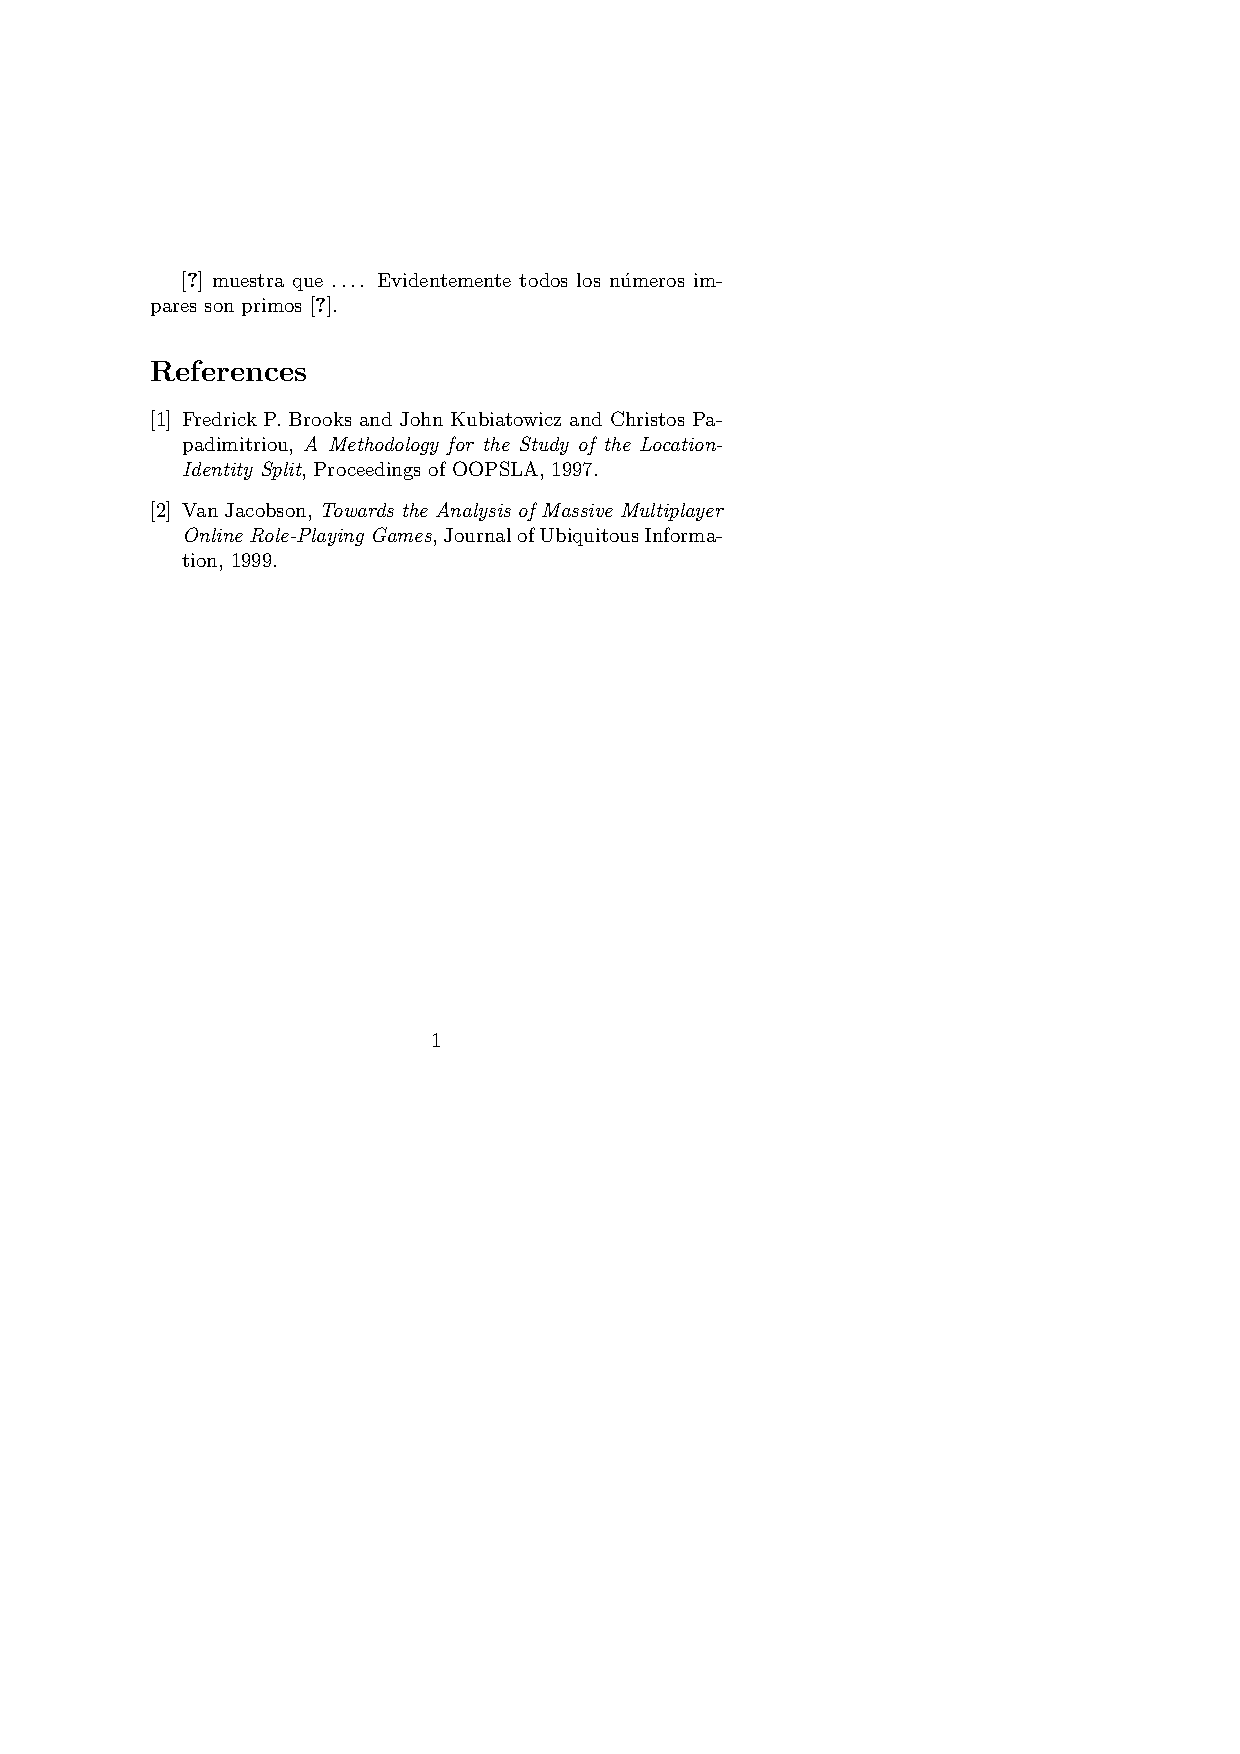
\includegraphics[width=\textwidth,clip,trim=1in 1.1in 1in 1.1in]{biblio-example.pdf}   
    \end{minipage}
    \end{itemize}
\end{frame}


\begin{frame}
  \begin{center}
    Gracias!
  \end{center}
\end{frame}

\end{document}
